\graphicspath{{1intro/asy/}}
\thispagestyle{empty}

\title{Math 120A --- Introduction to Group Theory}
\author{Neil Donaldson}
\date{Fall 2024}
\maketitle 


\section{Introduction: what is abstract algebra and why study groups?}\label{chap:intro}

To \emph{abstract} something means to remove context and application. Modern mathematics largely involves studying patterns and symmetries (often observed in the real world) abstractly so as to observe commonalities between structures in seemingly distinct places.\smallbreak

One reason to study groups is that they are relatively simple: a \emph{set} and a single \emph{operation} which together satisfy a few basic properties. Indeed you've been using this structure since Kindergarten!

\begin{example}{}{zadd}
	The integers $\Z=\{\ldots,-1,0,1,2,3,\ldots\}$ together with the operation $+$ form a group.
\end{example}

We'll see a formal definition shortly, at which point we'll be able to verify that $(\Z,+)$ really is a group. The simplicity of the group structure means that it is often used as a building block for more complicated structures.\footnote{For example, $\Z$ together with the two basic operations of addition and multiplication is a \emph{ring,} as you'll study in a later course.} Other reasons to study groups are their ubiquity and multitudinous applications. Here are just a few of the places where the language of group theory is essential.

\begin{description}
	\item[Permutations] The original use of \emph{group} was to describe the ways in which a set could be \emph{reordered.} Understanding permutations is of crucial importance to many areas of mathematics, particularly combinatorics, probability and Galois theory: this last, the crown jewel of undergraduate algebra, develops a deep relationship between the solvability of a polynomial and the \emph{permutation group} of its set of roots.
	\item[Geometry] Figures in Euclidean geometry (e.g.{} triangles) are \emph{congruent} if one may be transformed to the other by an element of the \emph{\href{https://en.wikipedia.org/wiki/Euclidean_group}{Euclidean group}} (\emph{a translation, rotation} or \emph{reflection}). More general geometries may also be described by their groups of symmetries. Groups may also be employed to describe geometric properties: for example, the number of holes in an object (a sphere has none, a torus one, etc.) is related to the structure of its \emph{\href{https://en.wikipedia.org/wiki/Fundamental_group}{fundamental group.}}
	\item[Chemistry] Group Theory may be applied to describe the symmetries of molecules and of crystalline substances.
	\item[Physics] Materials science sees group theory similarly to chemistry. Modern theories of the nature of the universe and fundamental particles/forces (e.g.{} gauge/string theories) also rely heavily on groups.
\end{description}

From the point of view of this course, the best reason to study groups is simply that they're \emph{fun}!

\begin{example}{}{motiv}
	To introduce the idea of abstraction, we consider what an equilateral triangle and the set $\{1,2,3\}$ have in common.\smallbreak
	The obvious answer is the number \emph{three,} but we can say a lot more. Both objects have \emph{symmetries}: rotations/reflections of the triangle and permutations (rearrangements) of the set $\{1,2,3\}$. By considering \emph{compositions} of these symmetries, we shall see that the sets of such are essentially identical.%\vspace{-5pt}
	
	\boldinline{Permutations of $\{1,2,3\}$} These can be written as functions using \emph{cycle notation.}\footnotemark\ For instance, $(1\,2)$ is the \emph{function} which swaps 1 and 2, leaving 3 alone. The function $(1\,2\,3)$ permutes all three numbers:
	\[
		(1\,2):
		\begin{cases}
			1\mapsto 2\\
			2\mapsto 1\\
			3\mapsto 3
		\end{cases}
		\qquad\text{and}\qquad
		(1\,2\,3):
		\begin{cases}
			1\mapsto 2\\
			2\mapsto 3\\
			3\mapsto 1
		\end{cases}
	\]
	It is not hard to convince yourself that there are \emph{six distinct permutations} of $\{1,2,3\}$; for brevity, we use the symbols $e,\mu_1,\mu_2,\mu_3,\rho_1,\rho_2$.
	\[
		\begin{array}{c|c|c}
			\text{Identity: leave everything alone} & \text{Swap two numbers} & \text{Permute all three}\\\hline
			e=() & \mu_1=(2\,3) & \rho_1=(1\,2\,3)\\
			& \mu_2=(1\,3) & \rho_2=(1\,3\,2)\\
			& \mu_3=(1\,2) &
		\end{array}
	\]
	Since permutations are functions, we may compose them. For instance (remember to do $\rho_2$ first!),
	\[
		\mu_1\circ\rho_2=(2\,3)(1\,3\,2):
		\begin{cases}
			1\mapsto 3\mapsto 2\\
			2\mapsto 1\mapsto 1\\
			3\mapsto 2\mapsto 3
		\end{cases}
	\]
	The result is the same as that obtained by the permutation $(1\,2)=\mu_3$, whence we write
	\[
		\textcolor{red}{\mu_1}\circ\textcolor{blue}{\rho_2}=\textcolor{Green}{\mu_3}
	\]
	This is an \emph{algebraic statement}: two elements $\textcolor{red}{\mu_1}$, $\textcolor{blue}{\rho_2}$ have been combined using an operation $\circ$ to produce a third element $\textcolor{Green}{\mu_3}$. The full list of compositions may be assembled in a table; read the left column first, then the top row.\label{intro:table}
	\[
		\begin{array}{c||c|c|c|c|c|c}
			\circ & e & \rho_1 & \textcolor{blue}{\rho_2} & \mu_1 & \mu_2 & \mu_3\\
			 \hline\hline
			e & e & \rho_1 & \rho_2 & \mu_1 & \mu_2 & \mu_3\\
			\hline
			\rho_1 & \rho_1 & \rho_2 & e & \mu_3 & \mu_1 & \mu_2\\
			\hline
			\rho_2 & \rho_2 & e & \rho_1 & \mu_2 & \mu_3 & \mu_1\\
			\hline
			\textcolor{red}{\mu_1} & \mu_1 & \mu_2 & \textcolor{Green}{\mu_3} & e & \rho_1 & \rho_2\\
			\hline
			\mu_2 & \mu_2 & \mu_3 & \mu_1 & \rho_2 & e & \rho_1\\
			\hline
			\mu_3 & \mu_3 & \mu_1 & \mu_2 & \rho_1 & \rho_2 & e
		\end{array}
	\]
	You should verify a few more of these yourself.
\end{example}

\vspace{-12pt}

\footnotetext{We will return to this notation in Chapter \ref{chap:perm}, so don't feel you have to be an expert now. The permutation $(1\,2)$ is known as a \emph{2-cycle} because it permutes two objects. The permutation $(1\,2\,3)$ is similarly a \emph{3-cycle.}}

\clearpage
\goodbreak


\begin{tcolorbox}[exstyle]
	\boldinline{The Equilateral Triangle}
	What does all this have to do with a triangle?\medbreak
	
	If we label the vertices of an equilateral triangle 1, 2, 3, then the above permutations correspond to \emph{symmetries} of the triangle: $\rho_1$ and $\rho_2$ are rotations, while each $\mu_i$ performs a reflection in the altitude through vertex $i$.\medbreak
	
	\begin{minipage}{0.64\textwidth}\vspace{0pt}
		The two sets of symmetries apply to different objects, but the structure of their \emph{compositions} are identical. For example, rotating the triangle clockwise (\textcolor{blue}{$\rho_2$}) followed by reflecting in the altitude through the lower-left corner (\textcolor{red}{$\mu_1$}), results in the triangle being flipped upside down as if we had only performed a single reflection ($\textcolor{Green}{\mu_3}$).\medbreak
		
		What do we gain from this correspondence? Intuition, for one thing! There is an obvious qualitative difference between the \emph{rotations} $\rho_1,\rho_2$ and the \emph{reflections} $\mu_1,\mu_2,\mu_3$: since reflections flip the triangle upside down, it is completely obvious that composition of reflections produces a rotation! The corresponding idea that composition of 2-cycles makes a 3-cycle is not so clear.
	\end{minipage}
	\hfill
	\begin{minipage}{0.35\textwidth}\vspace{-8pt}
		\flushright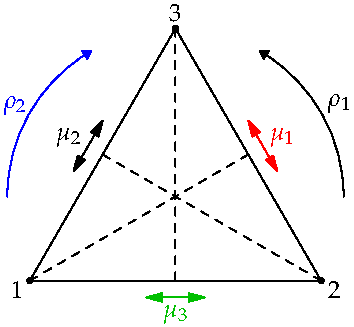
\includegraphics[scale=0.9]{intro-s3}
	\end{minipage}
	\medbreak
	
	Group theory, and abstract algebra more generally, is about ideas like this. By prioritizing abstract symmetries and patterns associated to objects over the objects themselves, unexpected connections between different part of mathematics are sometimes revealed.
	
	\boldinline{Summary} In this introductory example we considered two groups, which we now name.
	\begin{quote}
		$S_3$ is the \emph{symmetric group} on three letters: the permutations of $\{1,2,3\}$\smallbreak
		$D_3$ is the \emph{dihedral group} of order six: the symmetries of an equilateral triangle
	\end{quote}
	The mathematical way to summarize the relationship between these algebraic structures is to describe them as \emph{isomorphic},\footnotemark{} written $S_3\cong D_3$.
\end{tcolorbox}

As we progress, we'll see more examples of relationships between seemingly different structures. In the first half of the course (Chapters 2--5) our primary goal is develop familiarity with the most commonly encountered examples of groups so that they may quickly be recognized, even when well-disguised. The second half of the course is more abstract, with relatively few new examples of groups; comfort with the standard examples will be crucial in making sense of this harder material. 
% As as final motivation, consider the following questions:
% \begin{enumerate}
%   \item Label the faces of a cube with $1,\ldots,6$ dots as if to make a standard die. How many distinct dice can you make if each face has a different number of dots?
%   \item Repeat the experiment with a regular octahedron.
%   \item Join the midpoints of the faces of a cube: what happens? What does this have to do with questions 1 and 2?
%   \item Think about the same problem for a dodecahedron and an icosahedron.
% \end{enumerate}

\footnotetext{We will explain the term \emph{isomorphic} more concretely, and revisit both examples later. For the present, observe the use of the congruence symbol ($\cong$); given your understanding of congruent objects in geometry, think about why the use of this symbol isn't unreasonable.} 